\documentclass{article}

% content/resources/templates/preamble.tex
\usepackage[margin=0.6in]{geometry}
\author{Milav Dabgar}
\usepackage{amsmath,amssymb,amsthm}
\usepackage{booktabs}
\usepackage{multirow}
\usepackage{xcolor}
\usepackage{tcolorbox}
\tcbuselibrary{breakable,skins}
\usepackage[colorlinks=true,linkcolor=blue]{hyperref}
\usepackage{titlesec}
\usepackage{enumitem}
\usepackage{tikz}
\usepackage{pgfplots}
\usepackage{circuitikz}
\usepackage[version=4]{mhchem}
\usepackage{longtable}
\usepackage{array}
\usepackage{float}
\usepackage{caption}
\usepackage{listings}

\lstset{
  basicstyle=\small\ttfamily,
  breaklines=true,
  breakatwhitespace=false,
  postbreak=\mbox{\textcolor{red}{$\hookrightarrow$}\space},
  float=false,
  numbers=left,
  numberstyle=\tiny\color{gray},
  numbersep=10pt,
  xleftmargin=2em,
  keywordstyle=\color{blue},
  commentstyle=\color{green!60!black},
  stringstyle=\color{purple},
  backgroundcolor=\color{gray!5},
  showstringspaces=false,
  tabsize=2,
  captionpos=b,
  keepspaces=true,
  columns=flexible
}

\pgfplotsset{compat=1.18}
\usetikzlibrary{shapes,arrows,positioning,calc,patterns,decorations.pathmorphing,decorations.markings,arrows.meta}

% Color scheme
\definecolor{headcolor}{RGB}{0,102,204}
\definecolor{keycolor}{RGB}{220,20,60}
\definecolor{solutioncolor}{RGB}{34,139,34}
\definecolor{mnemoniccolor}{RGB}{148,0,211}
\definecolor{codecolor}{RGB}{0,0,100}

% Spacing
\setlength{\parskip}{3pt}
\setlist[itemize]{nosep}
\setlist[enumerate]{nosep}

% Title formatting
\titleformat{\section}{\Large\bfseries\color{headcolor}}{\thesection}{1em}{}
\titleformat{\subsection}{\large\bfseries\color{headcolor}}{\thesubsection}{1em}{}

% Pandoc tightlist compatibility
\providecommand{\tightlist}{%
  \setlength{\itemsep}{0pt}\setlength{\parskip}{0pt}}

% Pandoc longtable compatibility
\newcounter{none}
\def\thenone{}


% content/resources/templates/english-boxes.tex

% Custom environments
\newtcolorbox{solutionbox}{
 breakable,
 enhanced,
 colback=solutioncolor!5!white,
 colframe=solutioncolor!75!black,
 fonttitle=\bfseries,
 title=Solution
}

\newtcolorbox{solutionboxnobreak}{
 colback=solutioncolor!5!white,
 colframe=solutioncolor!75!black,
 fonttitle=\bfseries,
 title=Solution
}

\newtcolorbox{keyformula}{
 breakable,
 enhanced,
 colback=keycolor!5!white,
 colframe=keycolor!75!black,
 fonttitle=\bfseries,
 title=Key Formula
}

\newtcolorbox{mnemonicboxenv}{
 breakable,
 enhanced,
 colback=mnemoniccolor!5!white,
 colframe=mnemoniccolor!75!black,
 fonttitle=\bfseries,
 title=Mnemonic
}

\newcommand{\mnemonicbox}[1]{%
  \begin{mnemonicboxenv}
    #1
  \end{mnemonicboxenv}
}


% Custom commands for GTU solutions
% This file defines semantic commands for consistent formatting

% Question command with automatic formatting
\newcommand{\question}[2]{%
  \section*{Question #1}%
  \textbf{#2}%
}

% OR question variant
\newcommand{\questionor}[2]{%
  \section*{Question #1 OR}%
  \textbf{#2}%
}

% Proper table environment with caption
\newenvironment{answertable}[1]{%
  \begin{table}[htbp]
  \centering
  \caption{#1}
}{%
  \end{table}
}

% Proper figure environment for diagrams
\newenvironment{answerdiagram}[1]{%
  \begin{figure}[htbp]
  \centering
  \caption{#1}
}{%
  \end{figure}
}

% Semantic markup for key terms
\newcommand{\keyword}[1]{\textbf{#1}}
\newcommand{\code}[1]{\texttt{#1}}
\newcommand{\classname}[1]{\texttt{#1}}
\newcommand{\methodname}[1]{\texttt{#1}}

% Proper quotation marks
\newcommand{\mnemonic}[1]{``#1''}


\title{Fundamentals of Machine Learning (4341603) - Summer 2024 Solution}
\date{June 15, 2024}

\begin{document}
\maketitle

\questionmarks{1(a)}{3}{Define Machine Learning using suitable example?}
\begin{solutionbox}

Machine Learning is a subset of artificial intelligence that enables computers to learn and make decisions from data without being explicitly programmed for every task.

\begin{center}
\captionof{table}{Key Components of Machine Learning}
\begin{tabulary}{\linewidth}{L L}
\hline
\textbf{Component} & \textbf{Description} \\
\hline
\textbf{Data} & Input information used for training \\
\textbf{Algorithm} & Mathematical model that learns patterns \\
\textbf{Training} & Process of teaching the algorithm \\
\textbf{Prediction} & Output based on learned patterns \\
\hline
\end{tabulary}
\end{center}

\textbf{Example}: Email spam detection system learns from thousands of emails labeled as "spam" or "not spam" to automatically classify new emails.

\end{solutionbox}

\begin{mnemonicbox}
\mnemonic{Data Drives Decisions - Data trains algorithms to make intelligent decisions}
\end{mnemonicbox}

\questionmarks{1(b)}{4}{Explain the process of machine learning with the help of schematic representation}
\begin{solutionbox}

The machine learning process involves systematic steps from data collection to model deployment.

\begin{center}
\begin{tikzpicture}[node distance=1.5cm, auto]
    \node [gtu block] (Data) {Data Collection};
    \node [gtu block, below=0.8cm of Data] (Pre) {Data Preprocessing};
    \node [gtu block, below=0.8cm of Pre] (Feature) {Feature Selection};
    \node [gtu block, below=0.8cm of Feature] (Model) {Model Selection};
    \node [gtu block, below=0.8cm of Model] (Train) {Training};
    \node [gtu block, below=0.8cm of Train] (Valid) {Validation};
    \node [diamond, draw, aspect=2, below=1cm of Valid, align=center] (Check) {Performance\\OK?};
    \node [gtu block, below=1.5cm of Check] (Test) {Testing};
    \node [gtu block, below=0.8cm of Test] (Deploy) {Deployment};

    \path [gtu arrow] (Data) -- (Pre);
    \path [gtu arrow] (Pre) -- (Feature);
    \path [gtu arrow] (Feature) -- (Model);
    \path [gtu arrow] (Model) -- (Train);
    \path [gtu arrow] (Train) -- (Valid);
    \path [gtu arrow] (Valid) -- (Check);
    \path [gtu arrow] (Check) -- node[right] {Yes} (Test);
    \path [gtu arrow] (Check.east) -- ++(1,0) |- node[near start, right] {No} (Model.east);
    \path [gtu arrow] (Test) -- (Deploy);
\end{tikzpicture}
\captionof{figure}{Machine Learning Process}
\end{center}

\textbf{Process Steps:}
\begin{itemize}
    \item \keyword{Data Collection}: Gathering relevant dataset
    \item \keyword{Preprocessing}: Cleaning and preparing data
    \item \keyword{Training}: Teaching algorithm using training data
    \item \keyword{Validation}: Testing model performance
    \item \keyword{Deployment}: Using model for real predictions
\end{itemize}

\end{solutionbox}

\begin{mnemonicbox}
\mnemonic{Computers Can Truly Think - Collect, Clean, Train, Test}
\end{mnemonicbox}

\questionmarks{1(c)}{7}{Explain different types of machine learning with suitable application.}
\begin{solutionbox}

Machine learning algorithms are categorized based on learning approach and available data.

\begin{center}
\captionof{table}{Types of Machine Learning}
\begin{tabulary}{\linewidth}{L L L L}
\hline
\textbf{Type} & \textbf{Learning Method} & \textbf{Data Requirement} & \textbf{Example Application} \\
\hline
\textbf{Supervised} & Uses labeled data & Input-output pairs & Email classification \\
\textbf{Unsupervised} & Finds hidden patterns & Only input data & Customer segmentation \\
\textbf{Reinforcement} & Learns through rewards & Environment feedback & Game playing AI \\
\hline
\end{tabulary}
\end{center}

\textbf{Applications:}
\begin{itemize}
    \item \textbf{Supervised Learning}: Medical diagnosis, image recognition, fraud detection
    \item \textbf{Unsupervised Learning}: Market research, anomaly detection, recommendation systems
    \item \textbf{Reinforcement Learning}: Autonomous vehicles, robotics, strategic games
\end{itemize}

\begin{center}
\begin{tikzpicture}[node distance=1.5cm]
    \node [gtu block] (Root) {Machine Learning};
    
    \node [gtu block, below left=1.5cm and 1cm of Root] (Super) {Supervised};
    \node [gtu block, below=1.5cm of Root] (Unsuper) {Unsupervised};
    \node [gtu block, below right=1.5cm and 1cm of Root] (Reinf) {Reinforcement};
    
    \node [gtu state, below=0.8cm of Super, text width=2.5cm] (S1) {Classification\\Regression};
    \node [gtu state, below=0.8cm of Unsuper, text width=2.5cm] (U1) {Clustering\\Association};
    \node [gtu state, below=0.8cm of Reinf, text width=2.5cm] (R1) {Policy Learning\\Value Function};

    \path [gtu arrow] (Root) -- (Super);
    \path [gtu arrow] (Root) -- (Unsuper);
    \path [gtu arrow] (Root) -- (Reinf);
    \path [gtu arrow] (Super) -- (S1);
    \path [gtu arrow] (Unsuper) -- (U1);
    \path [gtu arrow] (Reinf) -- (R1);
\end{tikzpicture}
\captionof{figure}{Types of Machine Learning}
\end{center}

\end{solutionbox}

\begin{mnemonicbox}
\mnemonic{Students Usually Remember - Supervised, Unsupervised, Reinforcement}
\end{mnemonicbox}

\questionmarks{1(c) OR}{7}{What are various issues with machine learning? List three problems that are not to be solved using machine learning.}
\begin{solutionbox}

\begin{center}
\captionof{table}{Machine Learning Issues}
\begin{tabulary}{\linewidth}{L L L}
\hline
\textbf{Issue Category} & \textbf{Description} & \textbf{Impact} \\
\hline
\textbf{Data Quality} & Incomplete, noisy, biased data & Poor model performance \\
\textbf{Overfitting} & Model memorizes training data & Poor generalization \\
\textbf{Computational} & High processing requirements & Resource constraints \\
\textbf{Interpretability} & Black box models & Lack of transparency \\
\hline
\end{tabulary}
\end{center}

\textbf{Problems NOT suitable for ML:}
\begin{enumerate}
    \item \textbf{Simple rule-based tasks} - Basic calculations, simple if-then logic where rules are explicit.
    \item \textbf{Ethical decisions} - Moral judgments requiring human values and empathy (e.g., judicial sentencing).
    \item \textbf{Creative expression} - Original artistic creation requiring genuine human emotion and intent.
\end{enumerate}

\textbf{Other Issues:}
\begin{itemize}
    \item \keyword{Privacy concerns}: Sensitive data handling
    \item \keyword{Bias propagation}: Unfair algorithmic decisions
    \item \keyword{Feature selection}: Choosing relevant input variables
\end{itemize}

\end{solutionbox}

\begin{mnemonicbox}
\mnemonic{Data Drives Quality - Data quality directly affects model quality}
\end{mnemonicbox}

\questionmarks{2(a)}{3}{Give a summarized view of different types of data in a typical machine learning problem.}
\begin{solutionbox}

\begin{center}
\captionof{table}{Data Types in Machine Learning}
\begin{tabulary}{\linewidth}{L L L}
\hline
\textbf{Data Type} & \textbf{Description} & \textbf{Example} \\
\hline
\textbf{Numerical} & Quantitative values & Age: 25, Height: 170cm \\
\textbf{Categorical} & Discrete categories & Color: Red, Blue, Green \\
\textbf{Ordinal} & Ordered categories & Rating: Poor, Good, Excellent \\
\textbf{Binary} & Two possible values & Gender: Male/Female \\
\hline
\end{tabulary}
\end{center}

\textbf{Characteristics:}
\begin{itemize}
    \item \textbf{Structured}: Organized in tables (databases, spreadsheets)
    \item \textbf{Unstructured}: Images, text, audio files
    \item \textbf{Time-series}: Data points over time
\end{itemize}

\end{solutionbox}

\begin{mnemonicbox}
\mnemonic{Numbers Count Better Than Words - Numerical, Categorical, Binary, Text}
\end{mnemonicbox}

\questionmarks{2(b)}{4}{Calculate variance for both attributes. Determine which attribute is spread out around mean.}
\begin{solutionbox}

\textbf{Given Data:}
\begin{itemize}
    \item Attribute 1: 32, 37, 47, 50, 59
    \item Attribute 2: 48, 40, 41, 47, 49
\end{itemize}

\textbf{Calculations:}

\textbf{Attribute 1:}
\begin{itemize}
    \item Mean = $(32+37+47+50+59)/5 = 225/5 = 45$
    \item Variance = $[(32-45)^2 + (37-45)^2 + (47-45)^2 + (50-45)^2 + (59-45)^2]/5$
    \item Variance = $[169 + 64 + 4 + 25 + 196]/5 = 458/5 = 91.6$
\end{itemize}

\textbf{Attribute 2:}
\begin{itemize}
    \item Mean = $(48+40+41+47+49)/5 = 225/5 = 45$
    \item Variance = $[(48-45)^2 + (40-45)^2 + (41-45)^2 + (47-45)^2 + (49-45)^2]/5$
    \item Variance = $[9 + 25 + 16 + 4 + 16]/5 = 70/5 = 14$
\end{itemize}

\textbf{Result}: Attribute 1 (variance = 91.6) is more spread out than Attribute 2 (variance = 14).

\end{solutionbox}

\begin{mnemonicbox}
\mnemonic{Higher Variance Shows Spread - Greater variance indicates more dispersion}
\end{mnemonicbox}

\questionmarks{2(c)}{7}{List Factors that lead to data quality issue. How to handle outliers and missing values.}
\begin{solutionbox}

\begin{center}
\captionof{table}{Data Quality Issues}
\begin{tabulary}{\linewidth}{L L L}
\hline
\textbf{Factor} & \textbf{Cause} & \textbf{Solution} \\
\hline
\textbf{Incompleteness} & Missing data collection & Imputation techniques \\
\textbf{Inconsistency} & Different data formats & Standardization \\
\textbf{Inaccuracy} & Human/sensor errors & Validation rules \\
\textbf{Noise} & Random variations & Filtering methods \\
\hline
\end{tabulary}
\end{center}

\textbf{Handling Outliers:}
\begin{itemize}
    \item \textbf{Detection}: Statistical methods (Z-score, IQR)
    \item \textbf{Treatment}: Remove, transform, or cap extreme values
    \item \textbf{Visualization}: Box plots, scatter plots
\end{itemize}

\textbf{Handling Missing Values:}
\begin{itemize}
    \item \textbf{Deletion}: Remove incomplete records (rows with missing data)
    \item \textbf{Imputation}: Fill with mean, median, or mode
    \item \textbf{Prediction}: Use ML to predict missing values
\end{itemize}

\textbf{Code Example:}
\begin{lstlisting}[language=Python]
# Handle missing values
df.fillna(df.mean())  # Mean imputation
df.dropna()          # Remove missing rows
\end{lstlisting}

\end{solutionbox}

\begin{mnemonicbox}
\mnemonic{Clean Data Makes Models - Clean data produces better models}
\end{mnemonicbox}

\questionmarks{2(a) OR}{3}{Give different machine learning activities.}
\begin{solutionbox}

\begin{center}
\captionof{table}{Machine Learning Activities}
\begin{tabulary}{\linewidth}{L L L}
\hline
\textbf{Activity} & \textbf{Purpose} & \textbf{Example} \\
\hline
\textbf{Data Collection} & Gather relevant information & Surveys, sensors, databases \\
\textbf{Data Preprocessing} & Clean and prepare data & Remove noise, handle missing values \\
\textbf{Feature Engineering} & Create meaningful variables & Extract features from raw data \\
\textbf{Model Training} & Teach algorithm patterns & Use training dataset \\
\textbf{Model Evaluation} & Assess performance & Test accuracy, precision, recall \\
\textbf{Model Deployment} & Put model into production & Web services, mobile apps \\
\hline
\end{tabulary}
\end{center}

\textbf{Key Activities:}
\begin{itemize}
    \item \keyword{Exploratory Data Analysis}: Understanding data patterns
    \item \keyword{Hyperparameter Tuning}: Optimizing model settings
    \item \keyword{Cross-validation}: Robust performance assessment
\end{itemize}

\end{solutionbox}

\begin{mnemonicbox}
\mnemonic{Data Models Perform Excellently - Data preparation, Model building, Performance evaluation, Execution}
\end{mnemonicbox}

\questionmarks{2(b) OR}{4}{Calculate mean and median of the following numbers: 12,15,18,20,22,24,28,30}
\begin{solutionbox}

\textbf{Given numbers:} 12, 15, 18, 20, 22, 24, 28, 30

\textbf{Mean Calculation:}
Mean = $(12+15+18+20+22+24+28+30)/8 = 169/8 = 21.125$

\textbf{Median Calculation:}
\begin{itemize}
    \item Numbers are already sorted: 12, 15, 18, 20, 22, 24, 28, 30
    \item Even count (8 numbers)
    \item Median = (4th number + 5th number)/2 = $(20 + 22)/2 = 21$
\end{itemize}

\begin{center}
\captionof{table}{Statistical Summary}
\begin{tabulary}{\linewidth}{L L L}
\hline
\textbf{Measure} & \textbf{Value} & \textbf{Description} \\
\hline
\textbf{Mean} & 21.125 & Average value \\
\textbf{Median} & 21 & Middle value \\
\textbf{Count} & 8 & Total numbers \\
\hline
\end{tabulary}
\end{center}

\end{solutionbox}

\begin{mnemonicbox}
\mnemonic{Middle Makes Median - Middle value gives median}
\end{mnemonicbox}

\questionmarks{2(c) OR}{7}{Write a short note on dimensionality reduction and feature subset selection in context with data preprocessing.}
\begin{solutionbox}

\keyword{Dimensionality Reduction} removes irrelevant features and reduces computational complexity while preserving important information.

\begin{center}
\captionof{table}{Dimensionality Reduction Techniques}
\begin{tabulary}{\linewidth}{L L L}
\hline
\textbf{Technique} & \textbf{Method} & \textbf{Use Case} \\
\hline
\textbf{PCA} & Principal Component Analysis & Linear reduction \\
\textbf{LDA} & Linear Discriminant Analysis & Classification tasks \\
\textbf{t-SNE} & Non-linear embedding & Visualization \\
\textbf{Feature Selection} & Select important features & Reduce overfitting \\
\hline
\end{tabulary}
\end{center}

\textbf{Feature Subset Selection Methods:}
\begin{itemize}
    \item \keyword{Filter Methods}: Statistical tests, correlation analysis
    \item \keyword{Wrapper Methods}: Forward/backward selection
    \item \keyword{Embedded Methods}: LASSO, Ridge regression
\end{itemize}

\textbf{Benefits:}
\begin{itemize}
    \item \textbf{Computational Efficiency}: Faster training and prediction
    \item \textbf{Storage Reduction}: Less memory requirements
    \item \textbf{Noise Reduction}: Remove irrelevant features
    \item \textbf{Visualization}: Enable 2D/3D plotting
\end{itemize}

\begin{lstlisting}[language=Python]
from sklearn.decomposition import PCA
pca = PCA(n_components=2)
reduced_data = pca.fit_transform(data)
\end{lstlisting}

\end{solutionbox}

\begin{mnemonicbox}
\mnemonic{Reduce Features, Improve Performance - Fewer features often lead to better models}
\end{mnemonicbox}

\questionmarks{3(a)}{3}{Does bias affect the performance of the ML model? Explain briefly.}
\begin{solutionbox}

Yes, bias significantly affects ML model performance by creating systematic errors in predictions.

\begin{center}
\captionof{table}{Types of Bias}
\begin{tabulary}{\linewidth}{L L L}
\hline
\textbf{Bias Type} & \textbf{Description} & \textbf{Impact} \\
\hline
\textbf{Selection Bias} & Non-representative data & Poor generalization \\
\textbf{Confirmation Bias} & Favoring expected results & Skewed conclusions \\
\textbf{Algorithmic Bias} & Model assumptions & Unfair predictions \\
\hline
\end{tabulary}
\end{center}

\textbf{Effects on Performance:}
\begin{itemize}
    \item \keyword{Underfitting}: High bias leads to oversimplified models
    \item \keyword{Poor Accuracy}: Systematic errors reduce overall performance
    \item \keyword{Unfair Decisions}: Biased models discriminate against groups
\end{itemize}

\end{solutionbox}

\begin{mnemonicbox}
\mnemonic{Bias Breaks Better Performance - Bias reduces model effectiveness}
\end{mnemonicbox}

\questionmarks{3(b)}{4}{Compare cross-validation and bootstrap sampling}
\begin{solutionbox}

\begin{center}
\captionof{table}{Cross-validation vs Bootstrap Sampling}
\begin{tabulary}{\linewidth}{L L L}
\hline
\textbf{Aspect} & \textbf{Cross-validation} & \textbf{Bootstrap Sampling} \\
\hline
\textbf{Method} & Split data into folds & Sample with replacement \\
\textbf{Data Usage} & Uses all data & Creates multiple samples \\
\textbf{Purpose} & Model evaluation & Estimate uncertainty \\
\textbf{Overlap} & No overlap between sets & Allows duplicate samples \\
\hline
\end{tabulary}
\end{center}

\textbf{Key Differences:}
\begin{itemize}
    \item \textbf{Cross-validation}: Divides data into k equal parts. Trains on k-1 parts, tests on 1 part. Repeats k times.
    \item \textbf{Bootstrap Sampling}: Creates random samples with replacement. Generates multiple datasets of same size.
\end{itemize}

\end{solutionbox}

\begin{mnemonicbox}
\mnemonic{Cross Checks, Bootstrap Builds - Cross-validation checks performance, Bootstrap builds confidence}
\end{mnemonicbox}

\questionmarks{3(c)}{7}{Confusion Matrix Calculation and Metrics}
\begin{solutionbox}

\textbf{Given Information:}
\begin{itemize}
    \item True Positive (TP): 83
    \item False Positive (FP): 7
    \item False Negative (FN): 5
    \item True Negative (TN): 5
\end{itemize}

\begin{center}
\begin{tabulary}{\linewidth}{L L L}
\hline
 & \textbf{Predicted Buy} & \textbf{Predicted No Buy} \\
\hline
\textbf{Actually Buy} & 83 (TP) & 5 (FN) \\
\textbf{Actually No Buy} & 7 (FP) & 5 (TN) \\
\hline
\end{tabulary}
\end{center}

\textbf{Calculations:}

\textbf{a) Error Rate:}
Error Rate = $(FP + FN) / Total = (7 + 5) / 100 = 0.12 = 12\%$

\textbf{b) Precision:}
Precision = $TP / (TP + FP) = 83 / (83 + 7) = 83/90 = 0.922 = 92.2\%$

\textbf{c) Recall:}
Recall = $TP / (TP + FN) = 83 / (83 + 5) = 83/88 = 0.943 = 94.3\%$

\textbf{d) F-measure:}
F-measure = $2 \times (Precision \times Recall) / (Precision + Recall)$
F-measure = $2 \times (0.922 \times 0.943) / (0.922 + 0.943) = 0.932 = 93.2\%$

\end{solutionbox}

\begin{mnemonicbox}
\mnemonic{Perfect Recall Finds Everyone - Precision measures accuracy, Recall finds all positives}
\end{mnemonicbox}

\questionmarks{3(a) OR}{3}{Define in brief: a) Target function b) Cost function c) Loss Function}
\begin{solutionbox}

\begin{center}
\captionof{table}{Function Definitions}
\begin{tabulary}{\linewidth}{L L L}
\hline
\textbf{Function} & \textbf{Definition} & \textbf{Purpose} \\
\hline
\textbf{Target Function} & Ideal mapping from input to output & What we want to learn \\
\textbf{Cost Function} & Measures overall model error & Evaluate total performance \\
\textbf{Loss Function} & Measures error for single prediction & Individual prediction error \\
\hline
\end{tabulary}
\end{center}

\textbf{Relationship}: Cost function is typically the average of loss functions across all training examples.

\end{solutionbox}

\begin{mnemonicbox}
\mnemonic{Target Costs Less - Target function is ideal, Cost function measures overall error, Loss function measures individual error}
\end{mnemonicbox}

\questionmarks{3(b) OR}{4}{Explain balanced fit, underfit and overfit}
\begin{solutionbox}

\begin{center}
\captionof{table}{Model Fitting Types}
\begin{tabulary}{\linewidth}{L L L L}
\hline
\textbf{Fit Type} & \textbf{Training Error} & \textbf{Validation Error} & \textbf{Characteristics} \\
\hline
\textbf{Underfit} & High & High & Too simple model \\
\textbf{Balanced Fit} & Low & Low & Optimal complexity \\
\textbf{Overfit} & Very Low & High & Too complex model \\
\hline
\end{tabulary}
\end{center}

\begin{center}
\begin{tikzpicture}[node distance=2cm, auto]
    \node [gtu block] (Under) {Underfit\\(High Bias)};
    \node [gtu block, right=of Under] (Bal) {Balanced Fit\\(Optimal)};
    \node [gtu block, right=of Bal] (Over) {Overfit\\(High Variance)};
    
    \path [gtu arrow] (Under) -- (Bal);
    \path [gtu arrow] (Bal) -- (Over);
\end{tikzpicture}
\captionof{figure}{Model Complexity Spectrum}
\end{center}

\textbf{Solutions:}
\begin{itemize}
    \item \textbf{Underfit}: Increase model complexity, add features
    \item \textbf{Overfit}: Regularization, cross-validation, more data
\end{itemize}

\end{solutionbox}

\begin{mnemonicbox}
\mnemonic{Balance Brings Best Results - Balanced models perform best on new data}
\end{mnemonicbox}

\questionmarks{4(a)}{3}{Give classification learning steps.}
\begin{solutionbox}

\begin{center}
\captionof{table}{Classification Learning Steps}
\begin{tabulary}{\linewidth}{L L L}
\hline
\textbf{Step} & \textbf{Description} & \textbf{Purpose} \\
\hline
\textbf{Data Collection} & Gather labeled examples & Provide training material \\
\textbf{Preprocessing} & Clean and prepare data & Improve data quality \\
\textbf{Feature Selection} & Choose relevant attributes & Reduce complexity \\
\textbf{Model Training} & Learn from training data & Build classifier \\
\textbf{Evaluation} & Test model performance & Assess accuracy \\
\textbf{Deployment} & Use for new predictions & Practical application \\
\hline
\end{tabulary}
\end{center}

\end{solutionbox}

\begin{mnemonicbox}
\mnemonic{Data Preparation Facilitates Model Excellence - Data prep, Feature selection, Model training, Evaluation}
\end{mnemonicbox}

\questionmarks{4(b)}{4}{Linear Relationship Calculation}
\begin{solutionbox}

\textbf{Given Data:} Hours (X) vs Exam Score (Y)

\textbf{Linear Regression Calculation:}

\textbf{Step 1: Calculate means}
\begin{itemize}
    \item $\bar{X} = (2+3+4+5+6)/5 = 4$
    \item $\bar{Y} = (85+80+75+70+60)/5 = 74$
\end{itemize}

\textbf{Step 2: Calculate slope (b)}
\begin{itemize}
    \item Numerator = $\sum(X-\bar{X})(Y-\bar{Y}) = -60$
    \item Denominator = $\sum(X-\bar{X})^2 = 10$
    \item $b = -60/10 = -6$
\end{itemize}

\textbf{Step 3: Calculate intercept (a)}
\begin{itemize}
    \item $a = \bar{Y} - b\times\bar{X} = 74 - (-6)\times4 = 74 + 24 = 98$
\end{itemize}

\textbf{Linear Equation}: $Y = 98 - 6X$

\textbf{Interpretation}: For every additional hour of smartphone use, exam score decreases by 6 points.

\end{solutionbox}

\begin{mnemonicbox}
\mnemonic{More Phone, Less Score - Negative correlation between phone use and grades}
\end{mnemonicbox}

\questionmarks{4(c)}{7}{Explain classification steps in detail}
\begin{solutionbox}

Classification is a supervised learning process that assigns input data to predefined categories.

\textbf{Detailed Classification Steps:}

\textbf{1. Problem Definition}
\begin{itemize}
    \item Define classes and objectives
    \item Identify input features and target variable
\end{itemize}

\textbf{2. Data Collection and Preparation}
\begin{center}
\begin{tikzpicture}[node distance=1.2cm, auto]
    \node [gtu block] (Raw) {Raw Data};
    \node [gtu block, right=0.5cm of Raw] (Clean) {Data Clean};
    \node [gtu block, right=0.5cm of Clean] (Feat) {Features};
    \node [gtu block, right=0.5cm of Feat] (Split) {Split};
    
    \path [gtu arrow] (Raw) -- (Clean);
    \path [gtu arrow] (Clean) -- (Feat);
    \path [gtu arrow] (Feat) -- (Split);
\end{tikzpicture}
\end{center}

\textbf{3. Feature Engineering}
\begin{itemize}
    \item \textbf{Feature Selection}: Choose relevant attributes
    \item \textbf{Normalization}: Scale features to similar ranges
\end{itemize}

\textbf{4. Model Selection and Training}
\begin{center}
\captionof{table}{Common Classification Algorithms}
\begin{tabulary}{\linewidth}{L L L}
\hline
\textbf{Algorithm} & \textbf{Best For} & \textbf{Advantages} \\
\hline
\textbf{Decision Tree} & Interpretable rules & Easy to understand \\
\textbf{SVM} & High-dimensional data & Good generalization \\
\textbf{Neural Networks} & Complex patterns & High accuracy \\
\hline
\end{tabulary}
\end{center}

\textbf{5. Model Evaluation}
\begin{itemize}
    \item \textbf{Confusion Matrix}: Detailed performance analysis
    \item \textbf{Metrics}: Accuracy, Precision, Recall, F1-score
\end{itemize}

\textbf{6. Final Evaluation and Deployment}
\begin{itemize}
    \item Test on unseen data
    \item Deploy model for production use
\end{itemize}

\end{solutionbox}

\begin{mnemonicbox}
\mnemonic{Proper Data Modeling Evaluates Performance Thoroughly - Problem definition, Data prep, Modeling, Evaluation, Performance testing, Tuning}
\end{mnemonicbox}

\questionmarks{4(a) OR}{3}{Does the choice of the k value influence the performance of the KNN algorithm? Explain briefly}
\begin{solutionbox}

Yes, the k value significantly influences KNN algorithm performance.

\begin{center}
\captionof{table}{K Value Impact}
\begin{tabulary}{\linewidth}{L L L}
\hline
\textbf{K Value} & \textbf{Effect} & \textbf{Performance} \\
\hline
\textbf{Small K (k=1)} & Sensitive to noise & High variance, low bias \\
\textbf{Medium K} & Balanced decisions & Optimal performance \\
\textbf{Large K} & Smooth boundaries & Low variance, high bias \\
\hline
\end{tabulary}
\end{center}

\textbf{Selection Strategy:} Use cross-validation to find optimal k, often starting with $k = \sqrt{n}$.

\end{solutionbox}

\begin{mnemonicbox}
\mnemonic{Small K Varies, Large K Smooths - Small k creates variance, large k creates smooth boundaries}
\end{mnemonicbox}

\questionmarks{4(b) OR}{4}{Define Support Vectors in the SVM model.}
\begin{solutionbox}

Support Vectors are the critical data points closest to the decision boundary (hyperplane).

\begin{center}
\captionof{table}{Support Vector Characteristics}
\begin{tabulary}{\linewidth}{L L L}
\hline
\textbf{Aspect} & \textbf{Description} & \textbf{Importance} \\
\hline
\textbf{Location} & Closest points to hyperplane & Define decision boundary \\
\textbf{Distance} & Equal distance from boundary & Maximize margin \\
\textbf{Role} & Support the hyperplane & Determine optimal separation \\
\hline
\end{tabulary}
\end{center}

\begin{center}
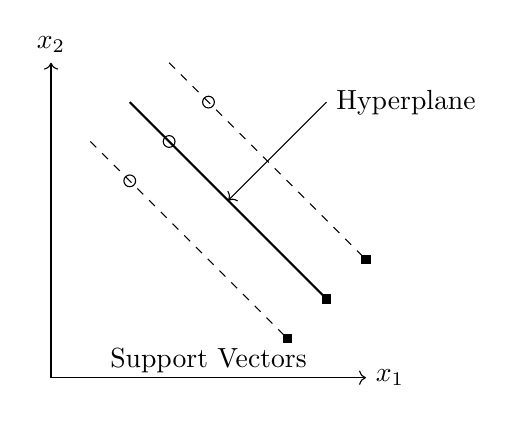
\begin{tikzpicture}
    % Axes
    \draw[->] (0,0) -- (4,0) node[right] {$x_1$};
    \draw[->] (0,0) -- (0,4) node[above] {$x_2$};
    
    % Points Class A (Circles)
    \foreach \p in {(1.5, 3), (2, 3.5), (1, 2.5)}
        \node[circle, draw, fill=white, inner sep=1.5pt] at \p {};
        
    % Points Class B (Crosses/Filled) - Using filled squares for B
    \foreach \p in {(3.5, 1), (3, 0.5), (4, 1.5)}
        \node[rectangle, draw, fill=black, inner sep=1.5pt] at \p {};
        
    % Support Vectors (closest ones)
    % A: (2.5, 2.5) approx
    % B: (3.5, 1.5) approx
    
    % Hyperplane y = -x + 4.5  (passing through 2.25, 2.25)
    \draw[thick] (1, 3.5) -- (3.5, 1);
    
    % Margins
    \draw[dashed] (0.5, 3) -- (3, 0.5);
    \draw[dashed] (1.5, 4) -- (4, 1.5);
    
    % Labels
    \node[right] at (3.5, 3.5) {Hyperplane};
    \draw[->] (3.5, 3.5) -- (2.25, 2.25);
    \node[below] at (2,0.5) {Support Vectors};
\end{tikzpicture}
\captionof{figure}{SVM Hyperplane and Support Vectors}
\end{center}

\end{solutionbox}

\begin{mnemonicbox}
\mnemonic{Support Vectors Support Decisions - These vectors support the decision boundary}
\end{mnemonicbox}

\questionmarks{4(c) OR}{7}{Explain logistic regression in detail.}
\begin{solutionbox}

Logistic Regression is a statistical method used for binary classification.

\textbf{Mathematical Foundation:}
\textbf{Sigmoid Function:} $\sigma(z) = 1 / (1 + e^{-z})$ where $z = \beta_0 + \beta_1x_1 + ...$

\begin{center}
\captionof{table}{Linear vs Logistic Regression}
\begin{tabulary}{\linewidth}{L L L}
\hline
\textbf{Aspect} & \textbf{Linear Regression} & \textbf{Logistic Regression} \\
\hline
\textbf{Output} & Continuous values & Probabilities (0-1) \\
\textbf{Function} & Linear & Sigmoid (S-curve) \\
\textbf{Purpose} & Prediction & Classification \\
\textbf{Error} & Mean Squared Error & Log-likelihood \\
\hline
\end{tabulary}
\end{center}

\textbf{Key Components:}
\begin{itemize}
    \item \textbf{Logistic Function}: S-shaped curve mapping values to [0,1].
    \item \textbf{Decision Rule}: If $P(y=1|x) > 0.5$, classify as positive.
    \item \textbf{Training}: Uses Maximum Likelihood Estimation.
\end{itemize}

\textbf{Applications:} Medical diagnosis, Email spam detection, Credit approval.

\begin{lstlisting}[language=Python]
from sklearn.linear_model import LogisticRegression
model = LogisticRegression()
model.fit(X_train, y_train)
probabilities = model.predict_proba(X_test)
\end{lstlisting}

\end{solutionbox}

\begin{mnemonicbox}
\mnemonic{Sigmoid Squashes Infinite Input - Sigmoid function converts any real number to probability}
\end{mnemonicbox}

\questionmarks{5(a)}{3}{Write a short note on Matplotlib python library.}
\begin{solutionbox}

Matplotlib is a comprehensive Python library for creating visualizations.

\begin{center}
\captionof{table}{Matplotlib Key Features}
\begin{tabulary}{\linewidth}{L L L}
\hline
\textbf{Feature} & \textbf{Purpose} & \textbf{Example} \\
\hline
\textbf{Pyplot} & MATLAB-like interface & Line plots \\
\textbf{Formats} & Save in various formats & PNG, PDF, SVG \\
\textbf{Subplots} & Multiple plots in one figure & Grid layouts \\
\hline
\end{tabulary}
\end{center}

\textbf{Basic Usage:}
\begin{lstlisting}[language=Python]
import matplotlib.pyplot as plt
plt.plot(x, y)
plt.show()
\end{lstlisting}

\end{solutionbox}

\begin{mnemonicbox}
\mnemonic{Matplotlib Makes Pretty Plots - Essential tool for data visualization}
\end{mnemonicbox}

\questionmarks{5(b)}{4}{K-means clustering for two-dimensional data}
\begin{solutionbox}

\textbf{Given Points:} Two groups clearly separated.
Group 1: (2,3) to (8,3). Group 2: (25,20) to (30,20).

\textbf{Algorithm Steps:}
\textbf{Step 1: Initialize centroids}
C1 = (4, 3), C2 = (27, 20)

\textbf{Step 2: Assign points}
Points (2,3)...(8,3) are closer to C1.
Points (25,20)...(30,20) are closer to C2.

\textbf{Step 3: Update centroids}
New C1 = Average of Group 1 = (5, 3)
New C2 = Average of Group 2 = (27.5, 20)

\textbf{Final Clusters:}
Cluster 1: Left group points. Cluster 2: Right group points.

\end{solutionbox}

\begin{mnemonicbox}
\mnemonic{Centroids Attract Nearest Neighbors - Points join closest centroid}
\end{mnemonicbox}

\questionmarks{5(c)}{7}{Give functions and its use of Scikit-learn}
\begin{solutionbox}

\textbf{a) Data Preprocessing:}
\begin{itemize}
    \item \code{StandardScaler()}: Normalize features
    \item \code{train\_test\_split()}: Split dataset
\end{itemize}

\textbf{b) Model Selection:}
\begin{itemize}
    \item \code{GridSearchCV()}: Hyperparameter tuning
    \item \code{cross\_val\_score()}: Cross-validation
\end{itemize}

\textbf{c) Model Evaluation:}
\begin{itemize}
    \item \code{accuracy\_score()}: Overall accuracy
    \item \code{confusion\_matrix()}: Error analysis
    \item \code{classification\_report()}: Comprehensive metrics
\end{itemize}

\begin{lstlisting}[language=Python]
from sklearn.metrics import classification_report
print(classification_report(y_true, y_pred))
\end{lstlisting}

\end{solutionbox}

\begin{mnemonicbox}
\mnemonic{Preprocess, Select, Evaluate - Complete ML workflow in Scikit-learn}
\end{mnemonicbox}

\questionmarks{5(a) OR}{3}{List out the major features of Numpy.}
\begin{solutionbox}

NumPy is fundamental for scientific computing.

\begin{itemize}
    \item \textbf{N-dimensional Arrays}: Efficient array objects
    \item \textbf{Broadcasting}: Operations on different sized arrays
    \item \textbf{Linear Algebra}: Matrix operations
    \item \textbf{Random Numbers}: Statistical simulations
\end{itemize}

\end{solutionbox}

\begin{mnemonicbox}
\mnemonic{Numbers Need Numpy's Power - Essential for numerical computations}
\end{mnemonicbox}

\questionmarks{5(b) OR}{4}{K-means clustering for one-dimensional data}
\begin{solutionbox}

\textbf{Dataset:} {1,2,4,5,7,8,10,11,12,14,15,17}

\textbf{K-means (k=3):}
\begin{itemize}
    \item \textbf{Cluster 1}: {1, 2, 4, 5} (Centroid $\approx$ 3)
    \item \textbf{Cluster 2}: {7, 8, 10, 11, 12} (Centroid $\approx$ 9.6)
    \item \textbf{Cluster 3}: {14, 15, 17} (Centroid $\approx$ 15.3)
\end{itemize}

\end{solutionbox}

\begin{mnemonicbox}
\mnemonic{Groups Gather by Distance - Similar points form natural clusters}
\end{mnemonicbox}

\questionmarks{5(c) OR}{7}{Give function and its use of Pandas library}
\begin{solutionbox}

\textbf{a) Preprocessing:}
\begin{itemize}
    \item \code{read\_csv()}: Load data
    \item \code{head()}, \code{tail()}: View data
\end{itemize}

\textbf{b) Inspection:}
\begin{itemize}
    \item \code{info()}: Data types, memory
    \item \code{describe()}: Statistical summary
    \item \code{isnull()}: Check missing values
\end{itemize}

\textbf{c) Cleaning:}
\begin{itemize}
    \item \code{dropna()}, \code{fillna()}: Handle missing data
    \item \code{groupby()}: Aggregate data
\end{itemize}

\begin{lstlisting}[language=Python]
df = pd.read_csv('data.csv')
print(df.describe())
\end{lstlisting}

\end{solutionbox}

\begin{mnemonicbox}
\mnemonic{Pandas Processes Data Perfectly - Comprehensive data manipulation tool}
\end{mnemonicbox}

\end{document}
